
\documentclass{article}
\usepackage[utf8]{inputenc}

\usepackage{amssymb, amsmath, lmodern, units, icomma, color, graphicx, bbm, hyperref, pdfpages, csquotes, listings, subcaption, epstopdf}

\usepackage{caption}
\usepackage{blindtext}
\usepackage[inline]{enumitem}
\usepackage{minted}
\usemintedstyle{friendly}
\graphicspath{ {../Images/} }
%\usepackage{xcolor}

\setlength{\parindent}{0em}
\setlength{\parskip}{0.5em}

\graphicspath{ {images/} }

\begin{document}

\section*{Udda och Jämna Signaler}

Eftersom signaler kan betraktas som matematiska funktioner kan vi säga att vi
har udda och jämna signaler, precis som vi har jämna och udda funktioner.
En funktion kan vara jämn, udda eller inget utav dem.

En funktion $f$ är jämn om $f(x)$ är samma som $f(-x)$.
I den vänstra bilden här nedan ser du ett exempel på en jämn funktion,
$f(x)=\cos(x)$. Notera att vilken punkt du än tittar på i figur 6a här
nedan så gäller alltid  $f(x) = f(-x)$.

En funktion $f$ är udda om $f(-x)$ är samma som $-f(x)$. I den högra bilden
nedan ser du ett exempel på en udda funktion , $f(x)=sin(x)$.
Notera att vilken punkt du än tittar på i figur 6b här nedan så gäller
alltid $f(-x) = -f(x)$.

\begin{figure}[ht]
\centering
\begin{subfigure}{0.50\textwidth}
  \centering
  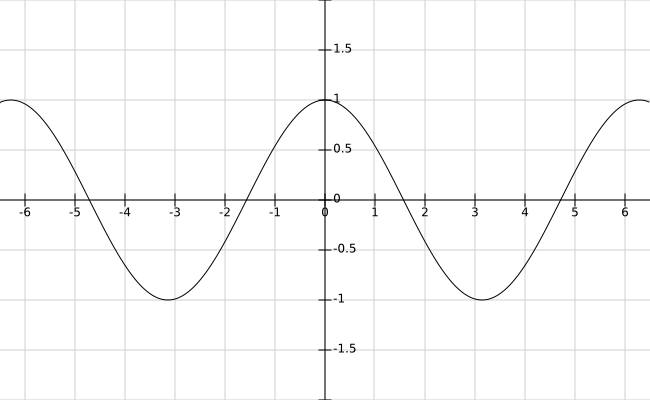
\includegraphics[width=0.90\linewidth]{image09.png}
  \caption{Jämn funktion}
  \label{}
\end{subfigure}%
\begin{subfigure}{0.50\textwidth}
  \centering
  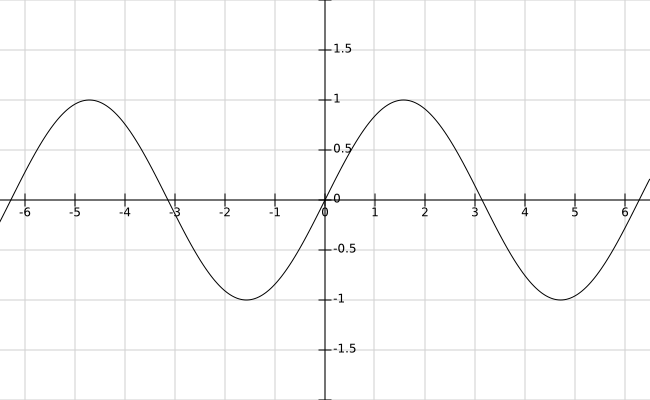
\includegraphics[width=0.90\linewidth]{image14.png}
  \caption{Udda funktion}
 \label{}
\end{subfigure}%
\caption{}
\label{}
\end{figure}



\begin{center}
Alltså:
\end{center}

Jämn funktion:\hfill Udda funktion:

$ f(x)=f(-x)$ \hfill $f(-x)=-f(x) $
\newline
\newline
Varför är det då bra att veta om en signal är jämn eller udda?
Mer om det kommer i avsnittet om Fourierserier!

\newpage

\textbf{Kryssfråga 8:} Är funktionen $f(t)=0.5\sin(2t)$ här nedan jämn,
udda eller ingetdera?
\begin{enumerate}[label={\alph*)},font={\bfseries}]
    \item Jämn
    \item Udda
    \item Ingetdera
\end{enumerate}

\begin{figure}[ht]
\centerline{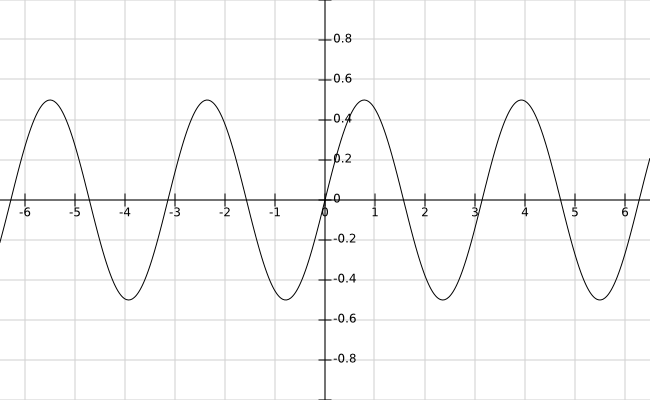
\includegraphics[scale=0.50]{image08.png}}
\caption{funktionen $f(t) = 0.5 \sin(2t)$}
\label{}
\end{figure}

\newpage

\textbf{Kryssfråga 9:} Är funktionen $f(t)=3\cos(0.25t)$ här nedan jämn, udda eller ingetdera?
\begin{enumerate}[label={\alph*)},font={\bfseries}]
    \item Jämn
    \item Udda
    \item Ingetdera
\end{enumerate}

\begin{figure}[ht]
\centerline{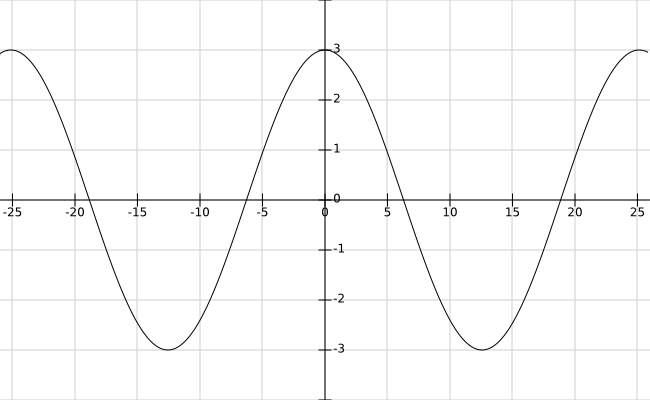
\includegraphics[scale=0.50]{image11.png}}
\caption{}
\label{}
\end{figure}

Då ska vi se hur man kan implementera det här! En funktion som avgör om en
signal är udda kan se ut så här:
\begin{minted}{haskell}
contIsOdd :: ContTimeFun -> ContTime -> Double -> Bool
contIsOdd signal step limit = and $ map testPair $ zip xs ys
    where testPair (a,b) = a ~= (-b)
          xs = map signal [0, step .. limit]
          ys = map signal [0,-step .. (-limit)]
\end{minted}

\textbf{Övning 7:} Implementera motsvarande funktion som undersöker
om en signal är jämn.\\

\textbf{Test:} Lös de två nedanstående uppgifter och kontrollera sedan svaret med
hjälp av programmet.\\

\textbf{Test 1:}
En signal har funktionen: $3*\sin(6t)$

Vad är signalens period?

Är signalen udda eller jämn?\\

\textbf{Test 2:}
En signal har funktionen: $\frac{1}{2} \cos(t)$

Vad är signalens period?

Är signalen udda eller jämn?\\

Testa gärna fler signaler!


\end{document}